
\section{Introduction}
\label{sec:intro}


% Edge Infrastructures are the next platform
With the emergence of Internet of Things (IoT) and augmented/virtual reality (AR/VR) 
applications, as well as the new usages related Network Function
Virtualization technologies (NFV), Cloud and Network communities are now advocating
for going towards massively distributed small sized infrastructures
that are deployed at the edge of the network.
%
Referred to as the Edge Computing paradigm, this model has been attracting
growing interest for the last few years as it enables delivering Cloud
Computing capabilities closer to end-users, their related devices, and the applications.
%

%% A lot of academics works focus on how to leverage these
%% infrastructures to address specicifc use-cases
While several academic studies have highlighted the advantages of Edge
Computing infrastructures in various
domains~\cite{bonomi2012fog,zhang2015cloud,yi2015fog,shi2016edge,satyanarayanan2017emergence},
the development of
%%  We need a resource management system that enables administrators to
%% operate and end-users to use edge resources.
a resource management system that will enable, on the one hand,
an operator to aggregate, supervise and expose such massively
distributed resources and, on the other hand, developers to implement
new kinds of services that may be deployed and managed on demand is
still an open question.

%%  Delivierng en Edge IaaS system is complex
Domain specific solutions such as ~\cite{bonomi2012fog} allow IoT applications 
to run on infrastructures composed of NFV-enabled hardware (at the edge) and
existing centralized clouds. However, these solutions do not allow to
run workloads in isolated environments such as containers or virtual
machines (VMs). 
%
This is rather critical as developers/end-users expect to find
most features that makes the success of current Cloud Computing solutions.

In 2016, the European Telecommunications Standards Institute (ETSI) MEC
Industry Specification Group defined  a software architecture
to orchestrate distinct independent cloud systems, \aka virtual
infrastructure managers in their terminology
(VIM)~\cite{7574435}. While the proposal should allow the deployment
of VMs at the edge, there is no implementation available yet.  At the
same time, a consortium composed of several industrial groups proposed
the ONAP framework~\cite{onap} that enables the orchestration and
automation of virtual network functions across distinct VIMs.  From
the academic side, federated approaches have been also investigated.
For instance, the FogBow proposal~\cite{brasileiro2016fogbow} aims to
support large federations of Infrastructure-as-a-service (IaaS) cloud
providers. More recently, the NIST Cloud Computing Program (NCCP)
%Public Working Group has recognized the importance of advancement and development of
%frameworks to support seamless implementation of federated community
%cloud environments. In August 2017, the NCCP
%Public Working Group
% (PWG) on Federated Cloud (PWGFC)
initiated a collaborative effort with the IEEE P2302 group (Standards for Intercloud Interoperability and
Federation), to advance Federated Cloud through the development
of a conceptual architecture and a vocabulary.
%The IEEE P2302 will
%develop a standard based on the NIST model.  Additional information
%can be found at
\footnote{\url{https://collaborate.nist.gov/twiki-cloud-computing/bin/view/CloudComputing/FederatedCloudPWGFC} (Valid on March 2018).}
%
While all these projects propose contributions to manage the life cycle of
geo-ditributed applications in a more software defined manner, they present two
weaknesses. First, they become more and more complex to finally
integrate most of the mechanisms that are already present in
IaaS resource management systems~\cite{}.\AL{Fix ref}  Second,
they have been designed by focusing on the developer/end-user's
requirements, that is without considering the administrator's
perspective.

Designing and implementing a complete software stack to enable
administrators to operate, and developers to use, distinct edge sites
like a global Cloud Computing infrastructure is a difficult challenge
for our community. However it is a challenge we should tackle soon to
favor the advent of the Edge Computing paradigm.

In this paper, we
present important reflections to consider before starting the development of such a system.
\begin{itemize}
\item First, we propose a classification of expected features from
  both administrators and end-users. Although this classification might be extended, it is already valuable to drive the design and implementation of a resource management system for the edge computing.
    \item Second, we discuss several design strategies. In particular, we
  analyze pros and cons of top/down and bottom up approaches. The
  former consists in interacting with each site only through the exposed APIs
  while the latter aims at revising internal mechanisms to enable
  native collaborations.
  \end{itemize}

\begin{figure}[t]
  \centering
  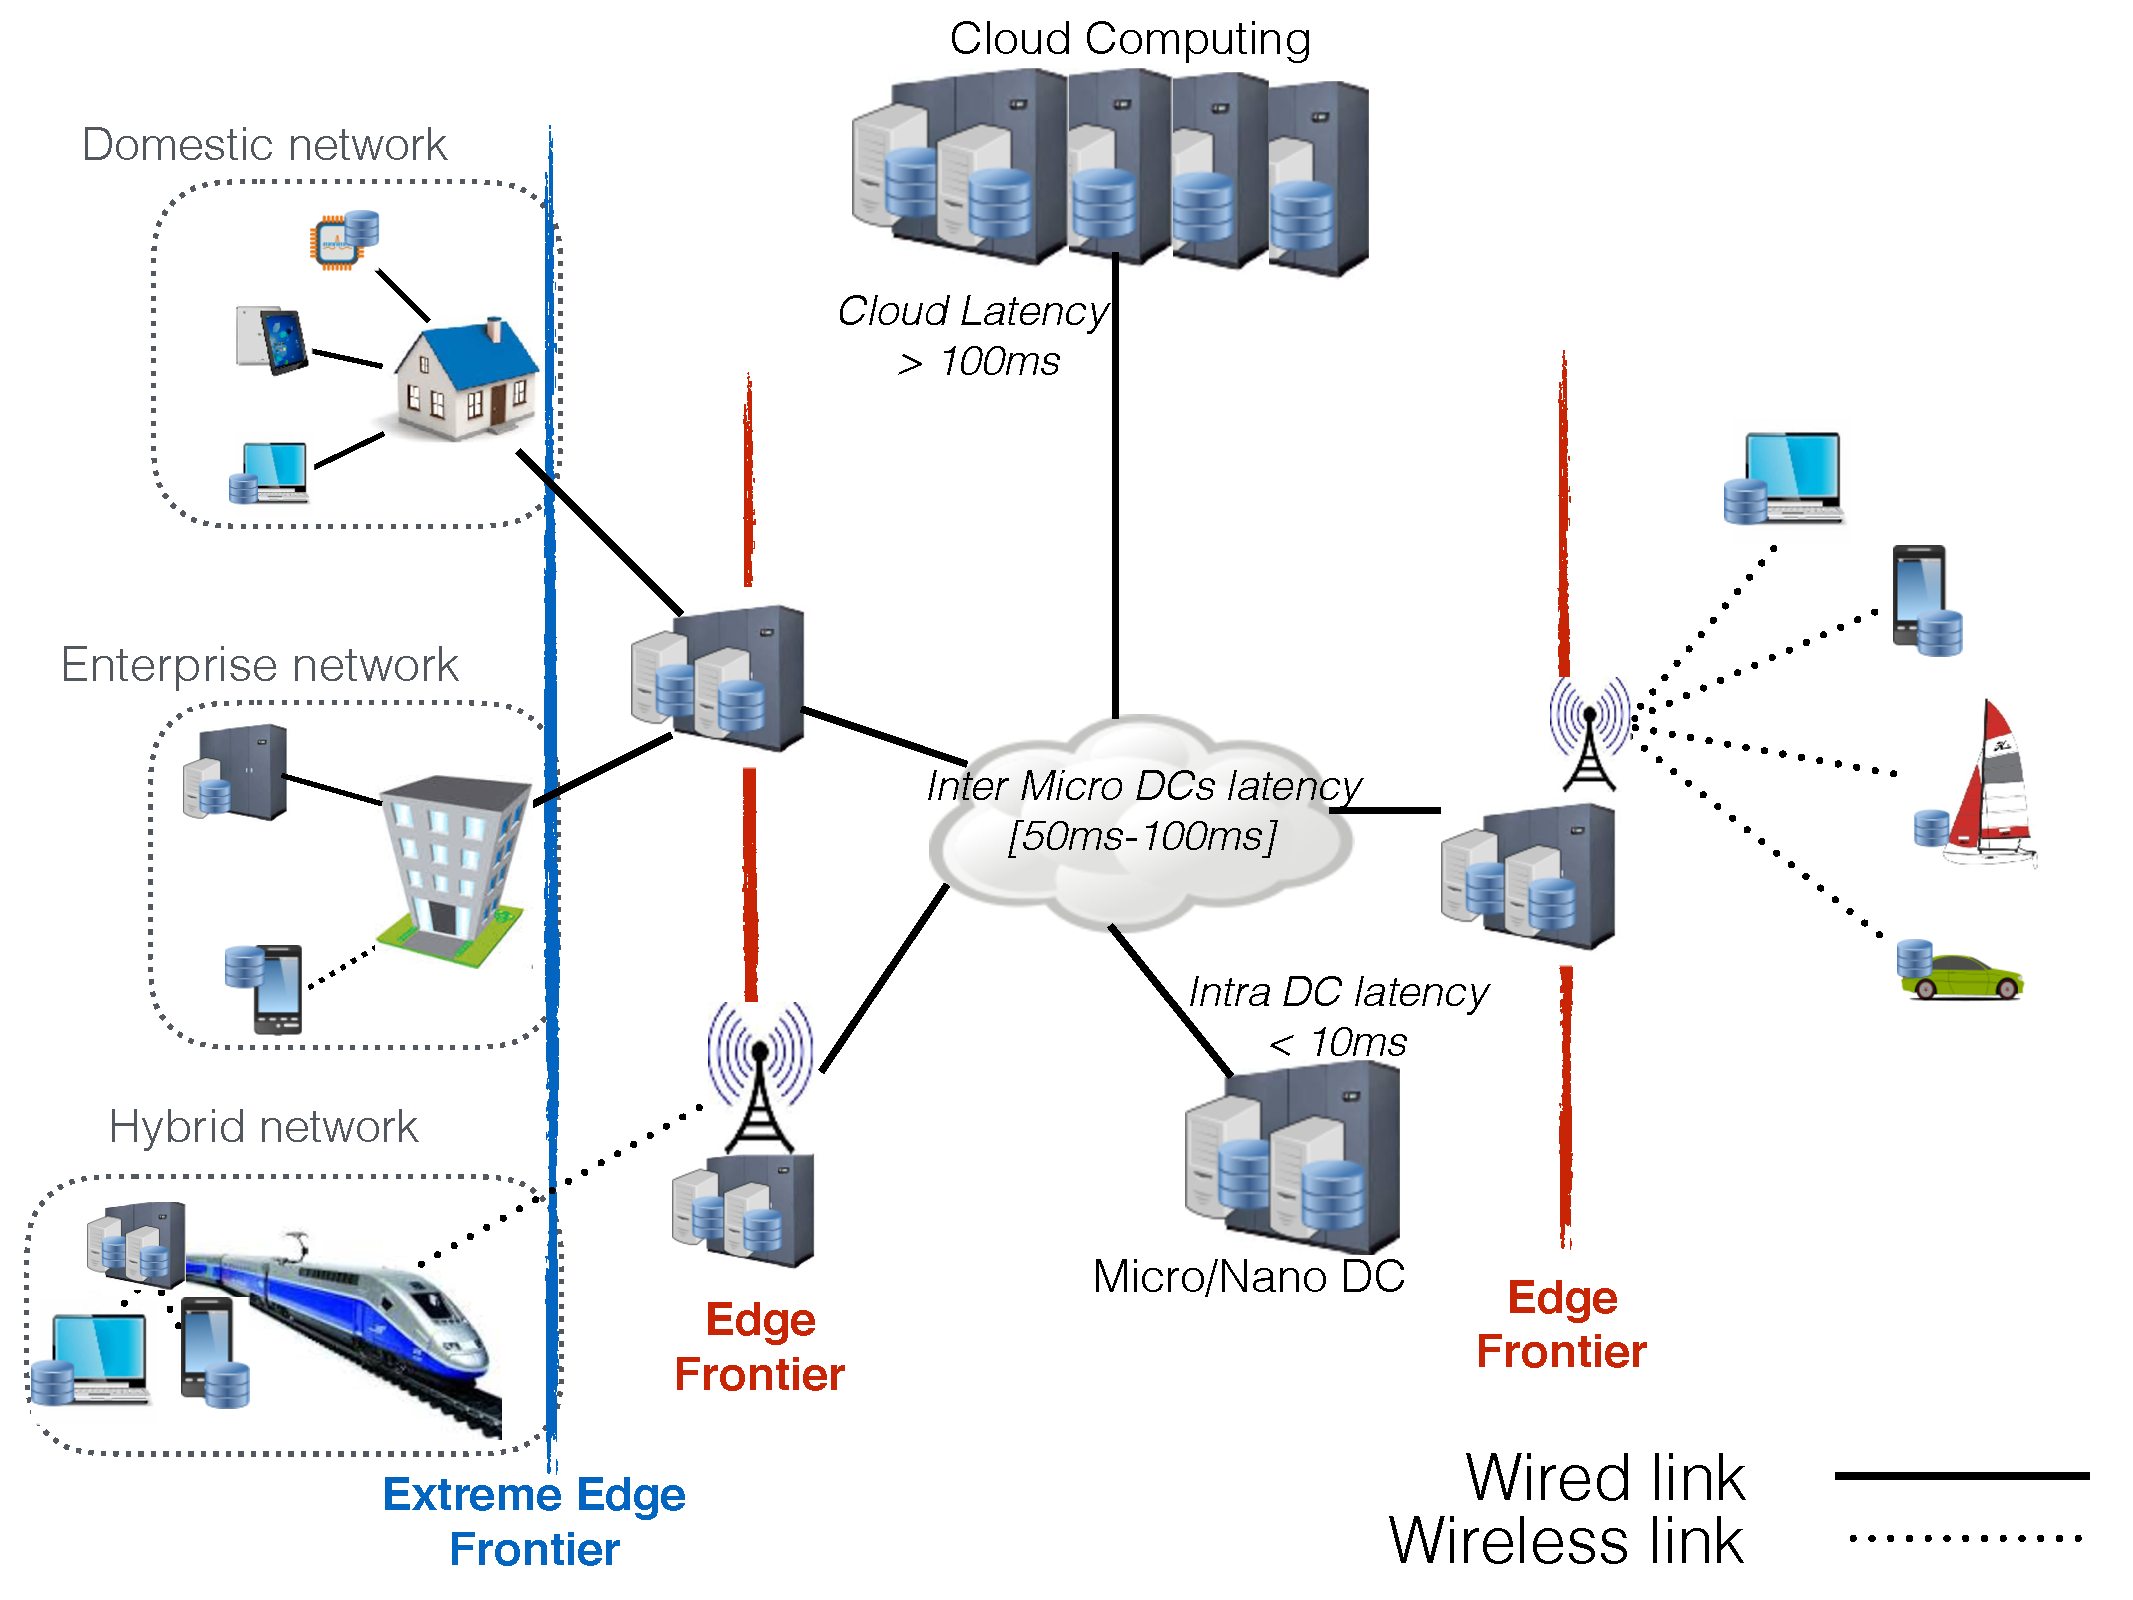
\includegraphics[width=\columnwidth]{./figures/figure_fog.pdf}
  \caption{An Edge Computing infrastructure composed of $4$ sites, built around
    micro/nano DCs~\cite{7923796}. It can be extended with Cloud Computing
    platforms when relevant (while farther, they provide more resources).
    The red dashed lines depicts a split-brain situation that isolates
    \emph{Site 1} from other sites.}
  \label{fig:fogedge-archi}
\end{figure}

Because there are as many edge infrastructures as use-cases, we
highlight that the edge infrastructure we considered to conduct this
study is composed from the hardware viewpoint of several
geo-distributed micro DCs (up to hundreds)\FW{AL: only hundreds? I would have said up to several tens of thousands}, which are themselves
composed of up to one hundred servers (up to two racks).
Figure~\ref{fig:fogedge-archi} gives an overview of this
infrastructure. The expected latency as well as the bandwidth between
each element may fluctuate significantly, in particular because the
network links can be either wired or wireless (represented by plain
and dashed lines on the figure). Moreover, short disconnections
between edge sites may occur leading to temporary network split brain
situations\AL{Add INFOCom citations}.  Finally, it might be possible
to consider additional micro DCs deployed at the Extreme Edge, within
private institutions or even public transports.
%
From the software point of view, in order to simplify the model and
without loss of generality, we mainly assume the OpenStack software
suite.  After seven years of intensive developments, OpenStack has
become the de facto open-source solution to operate, supervise and use
IaaS infrastructures.  The OpenStack community gathers more than 500
organizations, including large groups, in particular key actors of
edge infrastructures such as ATT, Verizon~\ldots.


The remainder of the paper is organized as
follows. Section~\ref{sec:requirements} presents major features
expected by administrators and developers, highlightling in particular
the main differences w.r.t federated infrastructures.
Section~\ref{sec:design_considerations} introduces two approaches that
open source communities could follow to design and develop an IaaS
toolkit, \aka a resource management system, dedicated to edge
environments. Section~\ref{sec:design_discussion} discusses pros/cons
of both approaches. Existing solutions that might serve as starting
points, are discussed in Section~\ref{sec:related_work}. Finally,
Section~\ref{sec:conclusion} concludes this paper.


% In this paper, we provide a list of expected features for both administrators and admins.
% We investigate whether a stack such as OpenStack, the defacto open-source standard can fullfil these requirements
% We finally discusss two possibles ways for moving forward: top/down vs bottom/up.

